\subsection{Javascript}

We use HTML, CSS and JavaScript build our frontend program. HTML and CSS describe the structure of the web page. We implement the user interface and data visualization function by JavaScript. JavaScript is a high-level, dynamic, untyped, and interpreted programming language.\cite{JS11} It is a multi-paradigm language, supports functional programming styles. We use JavaScript to implement this project because it is used such that we believe it is meaningful for computer engineer and computer scientist to learn it. What's more,  Java is an open source language such that all the best engines, tools, and libraries are open source. We can find useful functional program libraries. Although it is not a purely functional programming language, we can develop a functional styles program with functional programming libraries. In this project, we development our User Interface part by Lazy.js and the data visualizatoin part by Vis.js.

\subsubsection{Lazy.js}
Lazy.js is a utility library in a similar vein to Underscore or Lo-Dash, but with lazy evaluation.  Underscore or Lo-Dash provide a host of useful functions for array transformation: each function accepts an array as input,  does something with it and gives back a new array. However, the core of Lazy.js is function composition: each function accepts a function as input, stores it, and gives back an object that can do the same. 

It effectively changed the behavior of the input function, and that is why the performance of Lazy.js is better than Underscore and Lo-Dash. 
\begin{figure}[h]
\centering
		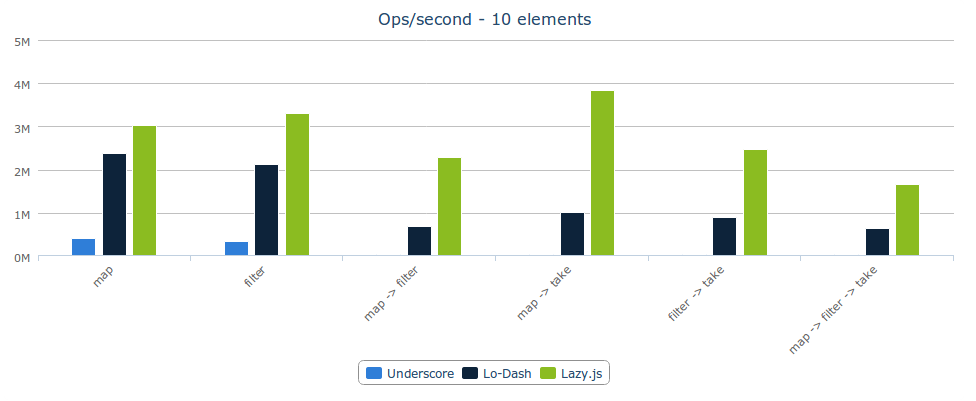
\includegraphics[width=\linewidth]{figure/lazy-performance}
	\caption{Lazy.js performance versus Underscore and Lo-Dash}
	\label{fig:lazy-performance}
\end{figure}

In this project, we mainly use two Lazy.js 's function: "map" and "reduce" to build some functional programming code. The map can create a new sequence whose values are calculated by passing this sequence's elements through some mapping function.  
Reduce can aggregate a sequence into a single value according to some accumulator function. 
\begin{figure}[h]
\centering
		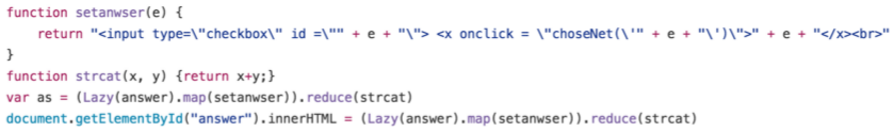
\includegraphics[width=\linewidth]{figure/mapreduce}
	\caption{code of Lazy.map and Lazy.reduce}
	\label{fig:mapreduce}
\end{figure}

As is shown in Figure 6, this code generates some checkbox and choice words,  where clicking the words will trigger a JavaScript function that will change the network. 
The function "setanswer()" takes a string(word) as input and return some HTML code that generates a checkbox and shows the words on the web page. The function "strcat()" catches two string. Thus "Lazy(answer).map(setanswer)" outputs the checkboxes and words the all the words in array "answer". Then we apply it with "Lazy().reduce(strcat)" to catch the HTML code for all words. The last step is embedding the code generate by "reduce" into HTML element with id "answer". The whole process do not influence other JavaScript variable. In other words, it is some functional programming code.

\subsubsection{Vis.js}
Vis.js is a dynamic, browser-based visualization library, which is easy to use and enable handling large amounts of dynamic data and manipulation the interaction with data.


\begin{figure}[h]
\centering
		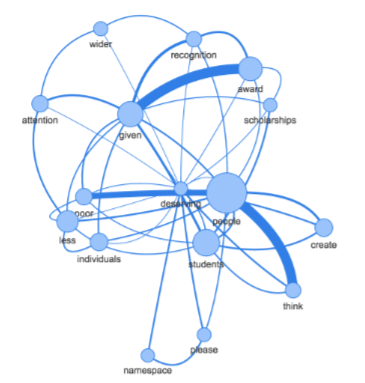
\includegraphics[width=\linewidth]{figure/VisNet}
	\caption{Network generated by Vis.js}
	\label{fig:netvis}
\end{figure}

We call "vis.Network()" funtion in our program when we want to show the network(such as the network in Figure 8) or refresh it. 


\begin{figure}[h]
\centering
		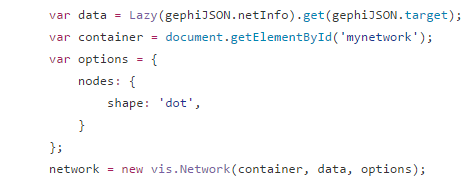
\includegraphics[width=\linewidth]{figure/Vis}
	\caption{code of Vis.network}
	\label{fig:vis}
\end{figure}

"vis.Network" is a visualization to display networks consisting of nodes and edges. As is shown in Figure 9, the function "vis.Network" takes 3 input parameters. The first one is container which is a CSS frame container that describes the position of the network. The second is the network data that parsed from JSON data imported from the server. The last parameter is the network option. Since our network is simple, we only need to set the shape of nodes as 'dot'. The front end program will generate a network on the CSS container with Id "mynetwork".